% !TEX root = main_min_disc_dist.tex
This section uses two benchmark models, double integrator and pursuit-evasion game, to exemplify the numerical properties of the MDR formulation. The double integrator model will be used to display the over-/under-approximation of the reachable set, as well as to compare policy iteration with value iteration. The pursuit-evasion game is used to demonstrate the advantages of multigridding. 

Unless stated otherwise all algorithms are initialized with $\vec{h}=\vec{l}-L$, and are considered converged when the distance (in the infinity norm) between consecutive iterates falls below $\epsilon =.0005$, i.e. $||\vec{U}^{k+1}$.

We present a double integrator example, with state $(x_1, x_2)$, control $u \in [u_{min}, u_{max}]$ and disturbance $d \in [d_{min}, d_{max}]$ with dynamics,
\begin{equation}
\begin{split}
\dot{x_1} & = x_2 \\
\dot{x_2} & = u \cdot(u_{max}-u_{min}) + u_{min} + d \cdot (d_{max}-d_{min}) + d_{min}
\end{split}
\end{equation}
In our experiments, we discretize the state space, to a $161 \times 161$ grid; control space and disturbance space. 

We first show, in Fig~\ref{fig:convergence} that $Z$ over approximates~(bold line) and under approximates~(dotted lines) the true reachable set~(shown in black) for two values of $\lambda = 0.1, 0.2$. The target set $\mathcal{T}$ is shown in red. 
\begin{figure}
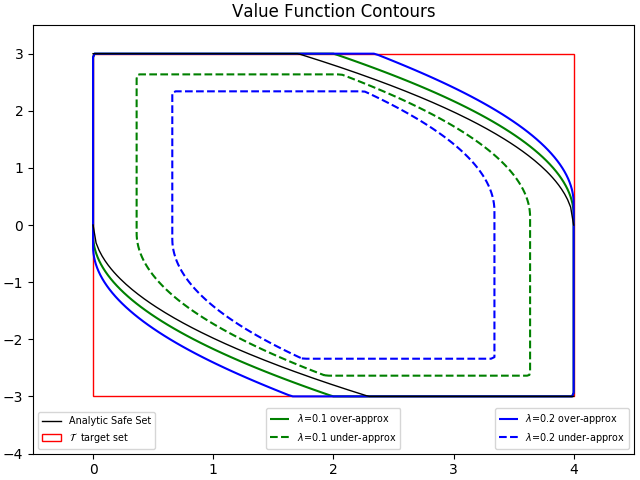
\includegraphics[scale=0.5]{convergence_difflambda.png}
\caption{The analytic reachable set $V$ and target set $\mathcal{T}$ are shown in black and red. The over and under approximated $Z_{\lambda}$ are shown in bold green and dotted green for $\lambda=0.1$; and bold blue and dotted blue line for $\lambda  = 0.2$. This suggests smaller the value of $\lambda$, the better $Z_{\lambda}$ approximates $V$.}
\label{fig:convergence}
\end{figure}

We next compare value iteration and policy iteration with increasing number of discrete actions in Table~\ref{tab:v_vs_p}. In the table we see that as the number of actions increase, there is sharp increase in how long value iteration takes to converge   while the increase is much smaller for policy iteration. However, the total time taken for policy iteration is much larger since there is a significant overhead in building the matrices for value functions. 
\begin{table}
\centering
\caption{Value Iteration vs Policy Iteration}
\label{tab:v_vs_p}
\begin{tabular}{|c| c| c| c|}
\hline
\# actions & VI & \multicolumn{2}{|c|}{Policy Iteration} \\ \cline{3-4}
 &  $T_{total} (Iters)$ & $T_{total}(Iters)$ & $T_{conv}$ \\ \hline
2 & 1.255 (204) & 68.793 (4) & 0.105 \\ \hline
50 &  7.562 (204)&  69.717 (4)& 0.365 \\ \hline
250 & 32.841 (204)&  251.39 (14)& 3.504 \\ \hline
500 & 63.815 (204)&  253.855 (14)& 6.741 \\
\hline
\end{tabular}
\end{table}

Finally, we ran value iteration from different initializations, the signed distance function $Z_0 = l(\cdot)$ and an all zeros $Z_0= 0$. The converged values functions had a norm of $0.000299$ between them, suggesting that MDR converges independent of the initialization. However, running MR with $V_0 = 0$, does not converge to the true value function.

% !TEX root = main_min_disc_dist.tex
\subsection{Pursuit-Evasion Game}

We now consider the pursuit-evasion game described in \cite{Mitchell2005}. In the game player I (the control) tries to avoid being captured by player II (the disturbance) on a two dimensional plane. Each player is modeled as a simple kinematic point object with planar position and heading, fixed linear velocity and controllable angular velocity. Taking player I to be at the origin the states $(x_1, x_2, x_3)$ are the relative position and heading of player II and the dynamics are

\begin{equation}
\begin{split}
&\dot{x_1}= -v_u+v_d \cos x_3 + ux_2\\ 
&\dot{x_2}= v_d \sin x_3 - ux_1\\ 
&\dot{x_3}= d-u
\end{split}
\end{equation}

The state space is over the domain $[-6,20] \times [-10,10] \times [0,2\pi[$ with $\U=[-u_{max},u_{max}]$ and $\D=[-d_{max}, d_{max}]$.

Player I is considered captured when the relative distance (in position) between both players is less than $R>0$, thus the target set is given by

\begin{equation}
\T= \{x| x_1^{2}+x_2^2 < R^2\}
\end{equation}


We first compute the value functions for the MR and MDR on a $41 \times 41 \times 41$ grid, and setting the model parameters to $v_u=v_d=5$, $u_{max}=d_{max}=1$, and $R=5$. This will be referred to as the nominal model $M_n$. A visualization of the zero sub-level set for both $V(x)$ and $Z(x)$ for $\lambda=0.001$ is shown in Fig.~\ref{fig:air3D}.


% \begin{figure}
% 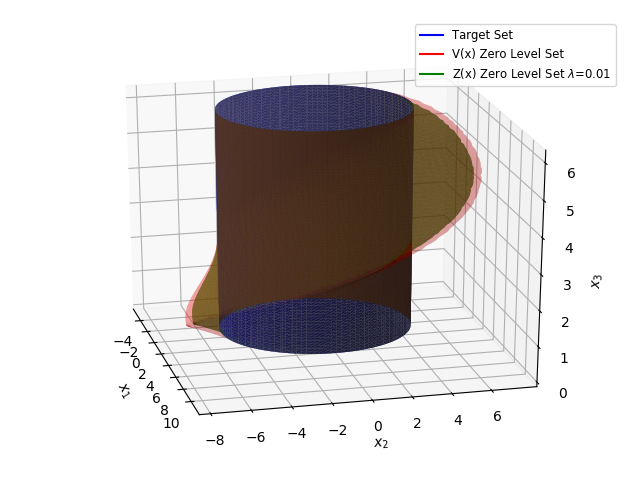
\includegraphics[trim= 2.5cm 0cm 0cm 0.5cm, clip=true,scale=0.65]{air_3D.png}
% \caption{The target set $\mathcal{T}$ is the blue cylinder. The zero sub-level sets of $V$ and $Z$ are in red and green, respectively. The discount rate is $\lambda=0.01$.}
% \label{fig:air3D}
% \end{figure}

\begin{figure*}[h]
    \centering
    \begin{subfigure}[t]{0.3\textwidth}
        \centering
        \includegraphics[trim= 4cm 0cm 0cm 0cm, scale=0.45]{air_3d_v1}
    \end{subfigure}%
    ~ 
    \begin{subfigure}[t]{0.3\textwidth}
        \centering
        \includegraphics[trim= 3cm 0cm 0cm 0cm, clip=true, scale=0.45]{air_3d_v2}
        %\caption{}
    \end{subfigure}
    ~
    \begin{subfigure}[t]{0.3\textwidth}
        \centering
        \includegraphics[trim= 3cm 0cm 0cm 0cm, clip=true, scale=0.45]{air_3d_v3}
        %\caption{}
    \end{subfigure}%
    \caption{The target set $\mathcal{T}$ (blue cylinder), zero sub-level sets of $V$ (red) and $Z$ (green) shown from three different perspectives. The discount rate for $Z$ is $\lambda=0.01$. Note that the zero sub-level set of $Z$ is a subset of the zero sub-level set of $V$.}
    \label{fig:air3D}
\end{figure*}

In the first experiment we compare a multigrid approach to value iteration.  The results are shown in Table~\ref{tab:multigrid_pe}. The experiment and table follows the same structure used for the double integrator model. Similar to the double integrator model, the multigrid approach outperforms value iteration for the pursuit-evasion game.

\begin{table}
\centering
\caption{Pursuit Evasion: Value iteration (VI) with Multigrid}
\begin{tabular}{|c| c| c| c| c| }
\hline
\# nodes & Coarse grid & Fine grid &  Fine grid with WS & Multigrid \\ \hline
$40^3$ & $2.068$ & $29.684$ & $24.320$ & $26.388$ \\ \hline
$80^3$ & $33.166$ & $352.099$ & $317.444$ & $350.610$\\ \hline
\end{tabular}
\label{tab:multigrid_pe}
\end{table}

We now construct two other models by tweaking $M_n$: setting $u_{max}=1.5$, which gives the evader an advantage, we get model $M_e$, and setting $d_{max}=1.5$, which gives the pursuer an advantage,  we get model $M_p$. In the final experiment we look at the impact of initializing value iteration with a solution from a similar model. Just like in the previous benchmark example, this experiment is motivated by Section \ref{sec:model_based}, where now $M_e$ and $M_p$ represent two possible models inferred from the system observations. In this context we have just ``learned" that the evader/pursuer is more maneuverable ($M_e$/$M_p$). We compute both value functions with and without setting the initialization to the solution for $M_n$. Again, we refer to this initialization as a warm start. The results are shown in Table~\ref{tab:ws_pe}.

\begin{table}
\centering
\caption{Pursuit Evasion: Value iteration (VI) with Warm Start (WS)}
\begin{tabular}{|c| c| c| c| c| c|}
\hline
\# nodes & $M_n$ & $M_e$ &  $M_e$ with WS & $M_p$ & $M_p$ with WS \\ \hline
$40^3$ & $35.043$ & $32.242$ & $21.483$ & $26.319$ & $23.366$ \\ \hline
$80^3$ & $439.751$ & $416.965$ & $308.821$ & $300.847$ & $296.568$\\ \hline
\end{tabular}
\label{tab:ws_pe}
\end{table}

